\documentclass[a4paper,14pt]{extarticle}

\usepackage[utf8x]{inputenc}
\usepackage[T1,T2A]{fontenc}
\usepackage[russian]{babel}
\usepackage{hyperref}
\usepackage{indentfirst}
\usepackage{here}
\usepackage{array}
\usepackage{graphicx}
\usepackage{caption}
\usepackage{subcaption}
\usepackage{chngcntr}
\usepackage{amsmath}
\usepackage{amssymb}
\usepackage{pgfplots}
\usepackage{pgfplotstable}
\usepackage[left=2cm,right=2cm,top=2cm,bottom=2cm,bindingoffset=0cm]{geometry}
\usepackage{multicol}

\renewcommand{\le}{\ensuremath{\leqslant}}
\renewcommand{\leq}{\ensuremath{\leqslant}}
\renewcommand{\ge}{\ensuremath{\geqslant}}
\renewcommand{\geq}{\ensuremath{\geqslant}}
\renewcommand{\epsilon}{\ensuremath{\varepsilon}}
\renewcommand{\phi}{\ensuremath{\varphi}}

\counterwithin{figure}{section}
\counterwithin{equation}{section}
\counterwithin{table}{section}
\newcommand{\sign}[1][5cm]{\makebox[#1]{\hrulefill}} % Поля подписи и даты
\graphicspath{{pics/}} % Путь до папки с картинками
\captionsetup{justification=centering,margin=1cm}
\def\arraystretch{1.3}

\usepackage{courier}

\usepackage{listings}
\lstset{ %
extendedchars=\true,
keepspaces=true,
language=C,						% choose the language of the code
basicstyle=\footnotesize,		% the size of the fonts that are used for the code
numbers=left,					% where to put the line-numbers
numberstyle=\footnotesize,		% the size of the fonts that are used for the line-numbers
stepnumber=1,					% the step between two line-numbers. If it is 1 each line will be numbered
numbersep=5pt,					% how far the line-numbers are from the code
backgroundcolor=\color{white},	% choose the background color. You must add \usepackage{color}
showspaces=false				% show spaces adding particular underscores
showstringspaces=false,			% underline spaces within strings
showtabs=false,					% show tabs within strings adding particular underscores
frame=single,           		% adds a frame around the code
tabsize=2,						% sets default tabsize to 2 spaces
captionpos=b,					% sets the caption-position to bottom
breaklines=true,				% sets automatic line breaking
breakatwhitespace=false,		% sets if automatic breaks should only happen at whitespace
escapeinside={\%*}{*)},			% if you want to add a comment within your code
postbreak=\raisebox{0ex}[0ex][0ex]{\ensuremath{\color{red}\hookrightarrow\space}},
texcl=true,
}

\lstset{basicstyle=\footnotesize\ttfamily,breaklines=true}

\begin{document}

\begin{titlepage}
\begin{center}
	\textbf{Санкт-Петербургский Политехнический Университет \\Петра Великого}\\[0.3cm]
	\small Институт компьютерных наук и технологий \\[0.3cm]
	\small Кафедра компьютерных систем и программных технологий\\[4cm]
	
	\textbf{ОТЧЕТ}\\ \textbf{о лабораторной работе}\\[0.5cm]
	\textbf{<<Использование стандартных подпрограмм для приближенного\\ вычисления интеграла>>}\\[0.1cm]
	\textbf{Вычислительная математика}\\[8.0cm]
\end{center}

\begin{flushright}
	\begin{minipage}{0.48\textwidth}
		\begin{flushleft}
			\small \textbf{Работу выполнил студент}\\[3mm]
			\small группа 23501/4 \hspace*{6mm} Дьячков В.В.\\[5mm]
			
			\small \textbf{Преподаватель}\\[5mm]
		 	\small \sign[3cm] \hspace*{5mm} к.т.н., доц. Цыган В.Н.\\[0.5cm]
		\end{flushleft}
	\end{minipage}
\end{flushright}

\vfill

\begin{center}
	\small Санкт-Петербург\\
	\small \the\year
\end{center}
\end{titlepage}

\section{Техническое задание}

\textbf{Вариант 7:} Для функции $f(x)$ по узлам $x_k$ построить интерполяционный полином Лагранжа $L(x)$ 10-й степени и сплайн функцию $S(x)$. Сравнить значения трех интегралов:

\begin{multicols}{3}
	\noindent 
	\[\int_0^3 f(x)dx\]
	\[\int_0^3 L(x)dx\]
	\[\int_0^3 S(x)dx\]
\end{multicols}

\section{Исходные данные}

Заданная функция: $f(x) = 1 - e^{-x}$

\vspace{0.3cm}

Узлы интерполяции: $x_k = 0.3 \cdot k\text{, для }k = 0, 1, ..., 10$

\section{Вычисление интегралов}

\subsection{Вычисление $\int f(x)dx$}

Аналитически найдем значение интеграла:
\vspace{-0.2cm}
\[
\int_0^3 f(x)dx = \int_0^3 \left(1 - e^{-x}\right) dx = \left.\left( x + e^{-x} \right)\right\vert_0^3 = 3 + e^{-3} - 1 \approx 2.04978706836786
\]

\subsection{Вычисление $\int L(x)dx$}

Для вычисления значения полинома Лагранжа в некоторой точке будем использовать подпрограмму \textbf{LAGRANGE}. Для вычисления интеграла $\int_0^3 L(x)dx$ будет использовать подпрограмму \textbf{quanc8} (см. листинг \ref{code:main}).

\subsection{Вычисление $\int S(x)dx$}

Для вычисления значения сплайн функции в некоторой точке будем использовать подпрограммы \textbf{SPLINE} для нахождения векторов \textbf{B, C, D} и \textbf{SEVAL} для вычисления значения сплайн функции. Для вычисления интеграла $\int_0^3 S(x)dx$ будем использовать подпрограмму \textbf{QUANC8} (см. листинг \ref{code:main}).

\section{Выполнение работы}

На рисунке \ref{fig:res} показан результат выполнения программы при $ABSERR = 10^{-14}$. В таблице в первом столбце указаны значения независимой переменной (между узлами интерполяции), во втором -- значения исходной функции, в третьем -- значения полинома Лагранжа, а в последнем -- значения сплайн функции.

После таблицы приведены значения трех интегралов, вычисленные при помощи подпрограммы \textbf{QUANC8}: $\int_0^3 f(x)dx$, $\int_0^3 L(x)dx$ и $\int_0^3 S(x)dx$. Можно заметить, что значения интеграла от исходной функции, вычсиленное аналитически, и значение интеграла, вычисленное с использованием подпрограммы \textbf{QUANC8}, совпадают.

В качестве вспомогательной информации приведены разности между интегралом от исходной функции и интегралом от полинома Лагранжа и сплайн функции.

\begin{figure}[H]
\begin{center}
	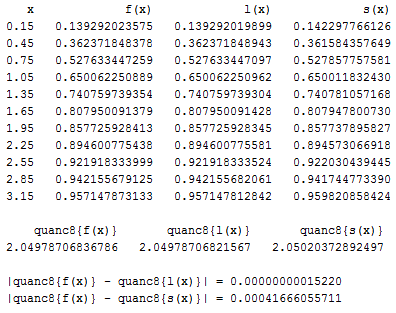
\includegraphics[width=0.58\textwidth]{output}
	\caption{Результат выполнения программы при $ABSERR = 10^{-14}$}
	\label{fig:res}
\end{center}
\end{figure}

\vspace{-1cm}

\section{Результаты}

Исследуем влияние значения $ABSERR$ на вычисление интеграла с помощью подпрограммы \textbf{QUANC8}. На рисунке \ref{fig:nofun} изображена зависимость количества вычислений функции в подпрограмме от значения абсолютной погрешности. Из графика видно, что при $ABSERR \approx 10^{-20}$ происходит сильное увеличение количества вычислений при расчете всех трех интегралов, а следовательно понижается производительность подпрограммы.

\begin{figure}[H]
\begin{center}
	\begin{tikzpicture} [every plot/.append style={thick}]
		\begin{axis}[
			height=0.35\textheight,
			width=0.85\textwidth,
			legend pos=north east,
			xlabel={$\lg ABSERR$},
			ylabel={$NOFUN$},
			xlabel near ticks,
			ylabel near ticks,
			xmax=10e2,
			xmin=10e-37,
			ymax=5e3,
			ymin=-500,
			xmode=log,
			log basis x=10,
			grid=major
		]
		\addplot table[x=abserr,y=nofun,col sep=comma]{data/f.csv};
		\addplot table[x=abserr,y=nofun,col sep=comma]{data/f-l.csv};
		\addplot table[x=abserr,y=nofun,col sep=comma]{data/f-s.csv};
		\legend{QUANC8(f(x)), QUANC8(L(x)), QUANC8(S(x))}
		\end{axis}
	\end{tikzpicture}
	\caption{Зависимость количества вычислений функции в подпрограмме \textbf{QUANC8} от абсолютной погрешности}
	\label{fig:nofun}
\end{center}
\end{figure}

На рисунке \ref{fig:f-l} изображена зависимость разности $\left| f(x) - L(x) \right|$ от задаваемой абсолютной погрешности подпрограммы \textbf{QUANC8}. На рисунке \ref{fig:errest-l} изображена зависимость оценочной погрешности от абсолютной погрешности. Из графика видно, что $ABSERR \le 10^{-14}$ оценочная погрешность близка к нулю. Пунктирной линией на графиках отмечено знанчение $ABSERR = 10^{-21}$, начиная с которого значение $FLAG$ становится ненулевым, т.е. при значениях меньше которого подпрограмма не завершается корректно.

\vspace{-0.5cm}

\begin{figure}[H]
\begin{center}
	\begin{tikzpicture} [every plot/.append style={thick}]
		\begin{axis}[
			height=0.34\textheight,
			width=0.85\textwidth,
			legend pos=north east,
			xlabel={$\lg ABSERR$},
			ylabel={$\left| f(x) - L(x) \right|$},
			xlabel near ticks,
			ylabel near ticks,
			xmax=10e2,
			xmin=10e-37,
			ymax=1.521965e-10,
			ymin=1.521936e-10,
			xmode=log,
			log basis x=10,
			grid=major,
			yticklabel style={/pgf/number format/fixed,/pgf/number format/precision=6},
		]
		\addplot table[x=abserr,y=f-l,col sep=comma]{data/f-l.csv};
		\addplot +[mark=none, dashed, black, samples=2] coordinates {(1e-21,1.521935e-10) (1e-21,1.521965e-10)};
		\end{axis}
	\end{tikzpicture}
	\caption{Зависимость разности $\left| f(x) - L(x) \right|$ от задаваемой абсолютной погрешности подпрограммы \textbf{QUANC8}}
	\label{fig:f-l}
\end{center}
\end{figure}

\vspace{-1.4cm}

\begin{figure}[H]
\begin{center}
	\begin{tikzpicture} [every plot/.append style={thick}]
		\begin{axis}[
			height=0.34\textheight,
			width=0.85\textwidth,
			legend pos=north east,
			xlabel={$\lg ABSERR$},
			ylabel={$\lg ERREST$},
			xlabel near ticks,
			ylabel near ticks,
			xmax=10e2,
			xmin=10e-37,
			ymax=10e-13,
			ymin=10e-21,
			xmode=log,
			log basis x=10,
			ymode=log,
			log basis y=10,
			grid=major,
			yticklabel style={/pgf/number format/fixed,/pgf/number format/precision=3},
		]
		\addplot table[x=abserr,y=errest,col sep=comma]{data/f-l.csv};
		\addplot +[mark=none, dashed, black, samples=2] coordinates {(1e-21,10e-21) (1e-21,10e-13)};
		\end{axis}
	\end{tikzpicture}
	\caption{Зависимость оценочной погрешности $ERREST$ от задаваемой абсолютной погрешности подпрограммы \textbf{QUANC8} при вычислении интеграла от полинома Лагранжа}
	\label{fig:errest-l}
\end{center}
\end{figure}

На рисунке \ref{fig:f-s} изображена зависимость разности $\left| f(x) - S(x) \right|$ от задаваемой абсолютной погрешности подпрограммы \textbf{QUANC8}. Из графика видно, что при $ABSERR \approx 10^{-7}$ происходит увеличение разности меджу интегралом от исходной функции и интегралом от сплайн-функции. На рисунке \ref{fig:errest-s} изображена зависимость оценочной погрешности от абсолютной погрешности. Из графика видно, что задание $ABSERR \le 10^{-20}$ перестает уменьшать оценочную погрешность $ERREST \approx 10^{-19}$. Пунктирной линией на графике отмечено знанчение $ABSERR = 10^{-25}$, начиная с которого $ERREST = 0$.

\vspace{-0.5cm}

\begin{figure}[H]
\begin{center}
	\begin{tikzpicture} [every plot/.append style={thick}]
		\begin{axis}[
			height=0.34\textheight,
			width=0.85\textwidth,
			legend pos=north east,
			xlabel={$\lg ABSERR$},
			ylabel={$\left| f(x) - S(x) \right|$},
			xlabel near ticks,
			ylabel near ticks,
			xmax=10e2,
			xmin=10e-37,
			ymax=4.2e-4,
			ymin=4.061e-4,
			xmode=log,
			log basis x=10,
			grid=major,
			yticklabel style={/pgf/number format/fixed,/pgf/number format/precision=3},
		]
		\addplot table[x=abserr,y=f-s,col sep=comma]{data/f-s.csv};
		\end{axis}
	\end{tikzpicture}
	\caption{Зависимость разности $\left| f(x) - S(x) \right|$ от задаваемой абсолютной погрешности подпрограммы \textbf{QUANC8}}
	\label{fig:f-s}
\end{center}
\end{figure}

\vspace{-1.5cm}

\begin{figure}[H]
\begin{center}
	\begin{tikzpicture} [every plot/.append style={thick}]
		\begin{axis}[
			height=0.34\textheight,
			width=0.85\textwidth,
			legend pos=north east,
			xlabel={$\lg ABSERR$},
			ylabel={$\lg ERREST$},
			xlabel near ticks,
			ylabel near ticks,
			xmax=10e2,
			xmin=10e-37,
			ymax=10e-4,
			ymin=10e-22,
			xmode=log,
			log basis x=10,
			ymode=log,
			log basis y=10,
			grid=major,
			yticklabel style={/pgf/number format/fixed,/pgf/number format/precision=3},
		]
		\addplot table[x=abserr,y=errest,col sep=comma]{data/f-s.csv};
		\addplot +[mark=none, dashed, black, samples=2] coordinates {(1e-24,10e-22) (1e-24,10e-4)};
		\end{axis}
	\end{tikzpicture}
	\caption{Зависимость оценочной погрешности $ERREST$ от задаваемой абсолютной погрешности подпрограммы \textbf{QUANC8} при вычислении интеграла от сплайн-функции}
	\label{fig:errest-s}
\end{center}
\end{figure}

\section{Выводы}

По полученным результатам вычисления интеграла $\int_0^3 f(x)dx$ можно сделать вывод, что в данном случае для его приближенного вычисления с использование подпрограммы \textbf{QUANC8} лучше использовать интерполяционный полином Лагрнджа. 

Помимо этого, на графиках \ref{fig:nofun}, \ref{fig:f-l} и \ref{fig:f-s} прослеживается закономерность: при задании меньшей абсолютной погрешности, подпрограмма выдает менее точный результат, если сравнивать его с аналитическим значением интеграла, используя при этом большее количество вычислений функции.

При этом из графика \ref{fig:errest-l} видно, что оценочная погрешность, начиная с которой уменьшение абсолютной погрешности не уменьшает оценчную, примерно равна $10^{-21}$, а из графика \ref{fig:errest-s} видно, что при абослютной погрешности меньшей или равной $10^{-25}$, оценочная погрешность равна нулю.

Таким образом, можно сделать вывод, что оптимальное значение абсолютной погрешности $ABSERR$ примерно равно $10^{-20}$ для полинома Лагрнжа и $10^{-25}$ для сплайн-функции, потому как большие значения приведут к увеличению оценочной погрешности, а уменьшение не даст более точного значения, только увеличит количество вычислений функции и даже приведет к некорректному завершению подпрограммы в случае с полиномом Лагранжа. 

\section*{Приложение}

\captionof{lstlisting}{main.cpp}
\lstinputlisting[
	basicstyle=\scriptsize,	
	numberstyle=\scriptsize,
	label=code:main
]{main.cpp}
\parindent=1cm

\end{document}
